% Possible supplemental figures
\begin{figure}[]
    \setfigurenum{S1}
    \centering
    \begin{minipage}{0.5\textwidth}
        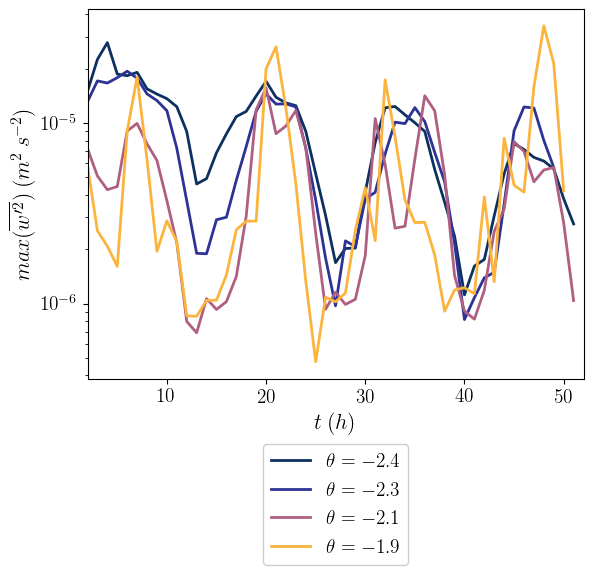
\includegraphics[width=\textwidth]{Figures/w2_max_cmp_dT_t.png}
    \end{minipage}%
    \begin{minipage}{0.5\textwidth}
        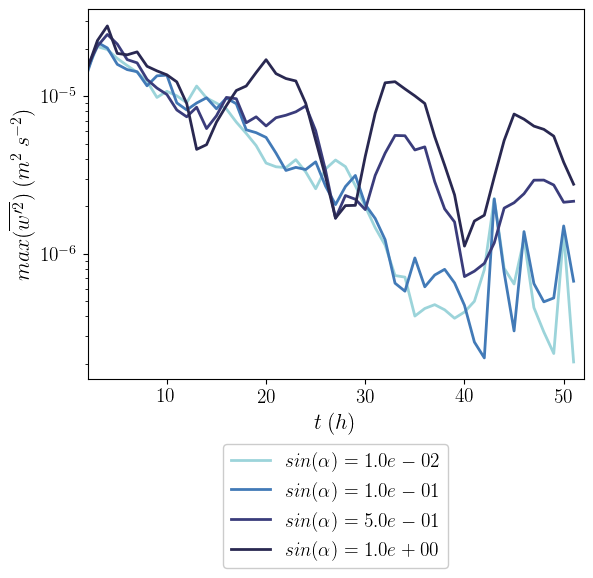
\includegraphics[width=\textwidth]{Figures/w2_max_cmp_dalpha_t.png}
    \end{minipage}
    \caption{Timeseries of maximum vertical velocity fluctuation per hour for (a) thermal driving cases and (b) slope cases.}
    \label{fig:max_w2_timeseries}
\end{figure}

\begin{figure}
    \centering
    \begin{minipage}{0.5\textwidth}
        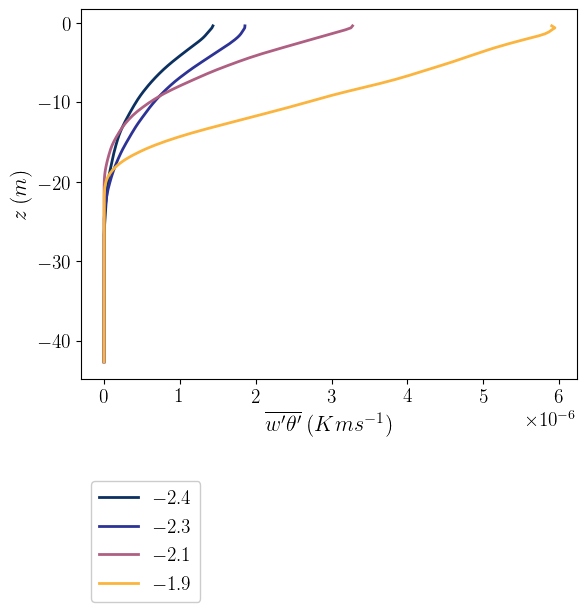
\includegraphics[trim={0 4cm 0 0},clip,width=\textwidth]{Figures/heatflux_cmp_dT_44h_tav12_z_profile.png}
    \end{minipage}%
    \begin{minipage}{0.5\textwidth}
        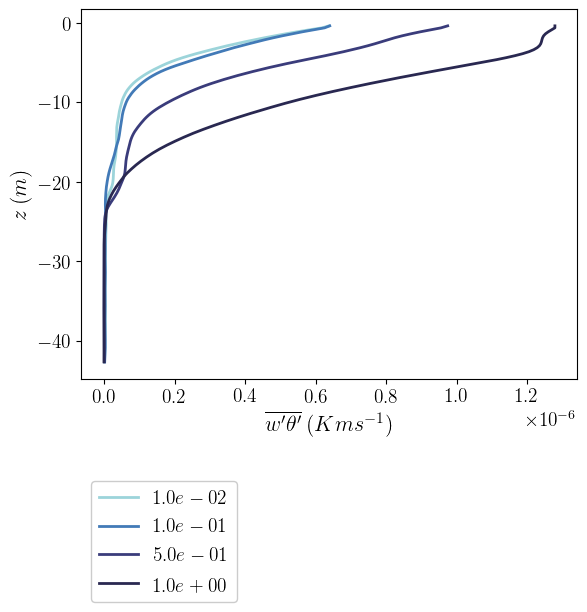
\includegraphics[trim={0 4cm 0 0},clip,width=\textwidth]{Figures/heatflux_cmp_slope_46h_tav12_z_profile.png}
    \end{minipage}
    \begin{minipage}{0.5\textwidth}
        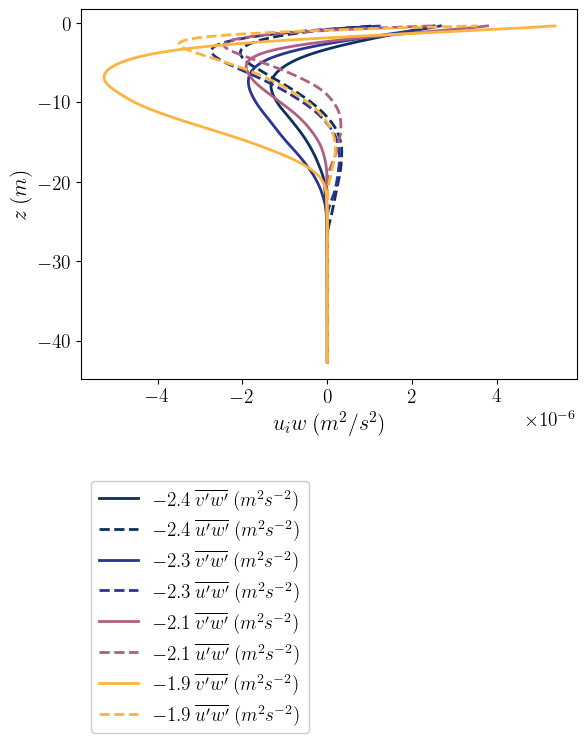
\includegraphics[trim={0 7.5cm 0 0},clip,width=\textwidth]{Figures/momflux_cmp_dT_44h_tav12_z_profile.png}
        \centering 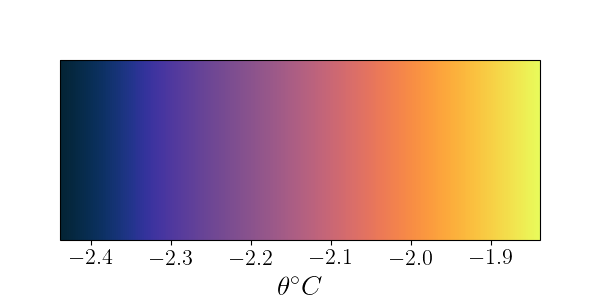
\includegraphics[width=0.7\textwidth,trim={1cm 0cm 1cm 5cm}, clip]{Figures/colorbar_thermal_driving.png}
    \end{minipage}%
    \begin{minipage}{0.5\textwidth}
        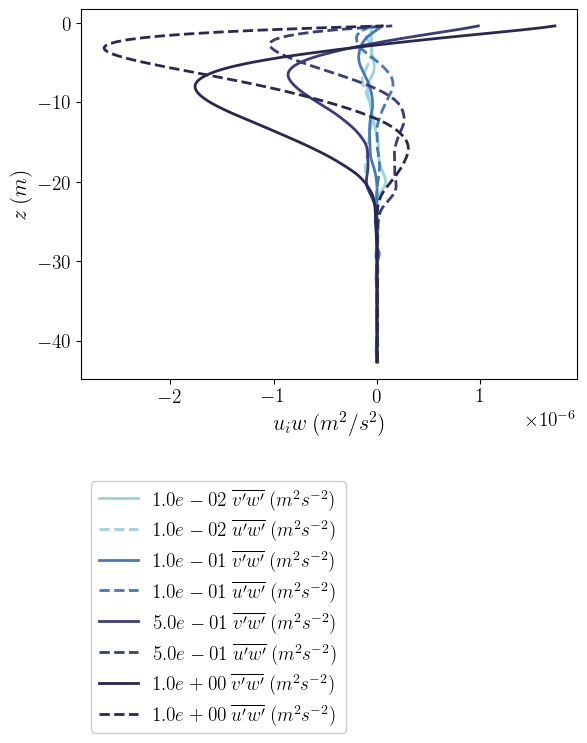
\includegraphics[trim={0 7.5cm 0 0},clip,width=\textwidth]{Figures/momflux_cmp_dslope_46h_tav12_z_profile.png}
        \centering 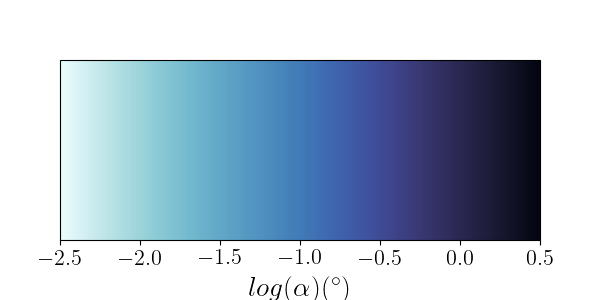
\includegraphics[width=0.7\textwidth,trim={1cm 0cm 1cm 5cm}, clip]{Figures/colorbar_slope.png}
    \end{minipage}
    \caption{Vertical profile of (a,b) heat flux and (c,d) momentum flux averaged over the last inertial period for (a,c) temperature cases and (b,d) slope cases. Momentum flux is expressed in two components:  $\overline{u'w'}$ (dashed) and $\overline{v'w'}$ (solid).} %Change the time interval in (b) back 2h to match (a)
    \label{fig:flux_profiles}
\end{figure}

\begin{figure}
    \centering
    \begin{minipage}{0.5\textwidth}
        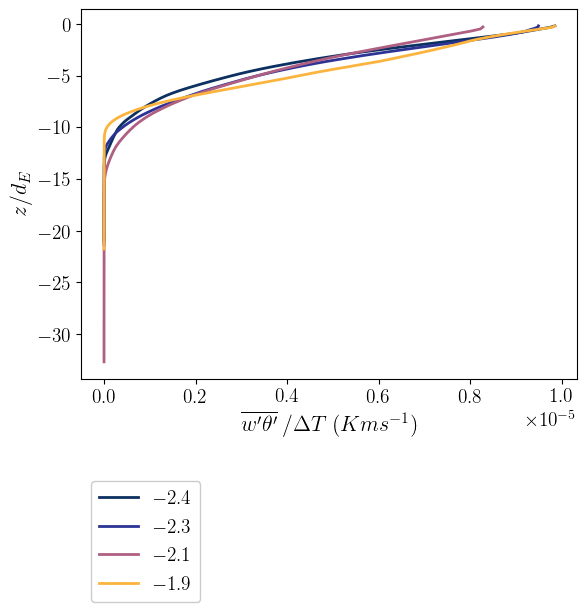
\includegraphics[trim={0 4cm 0 0},clip,width=\textwidth]{Figures/heatflux_cmp_dT_43h_tav13_dTscale_z_profile.png}
    \end{minipage}%
    \begin{minipage}{0.5\textwidth}
        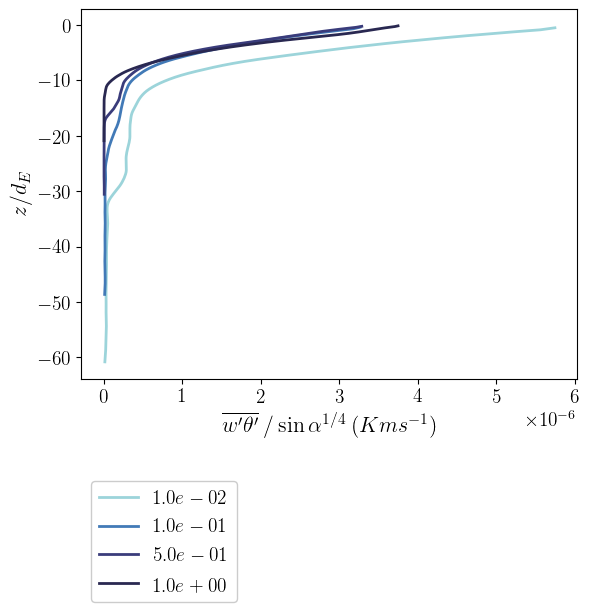
\includegraphics[trim={0 4cm 0 0},clip,width=\textwidth]{Figures/heatflux_cmp_slope_46h_tav13_slopescale_z_profile.png}
    \end{minipage}
    \begin{minipage}{0.5\textwidth}
        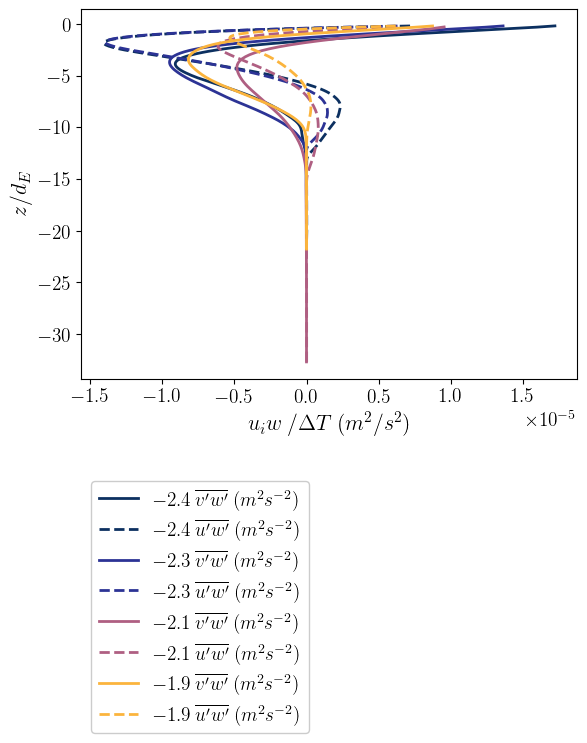
\includegraphics[trim={0 7.5cm 0 0},clip,width=\textwidth]{Figures/momflux_cmp_dT_43h_tav13_dTscale_z_profile.png}
        \centering 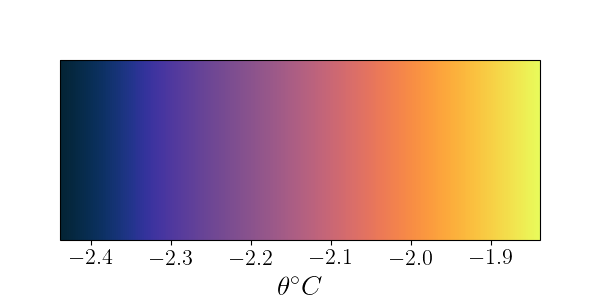
\includegraphics[width=0.7\textwidth,trim={1cm 0cm 1cm 5cm}, clip]{Figures/colorbar_thermal_driving.png}
    \end{minipage}%
    \begin{minipage}{0.5\textwidth}
        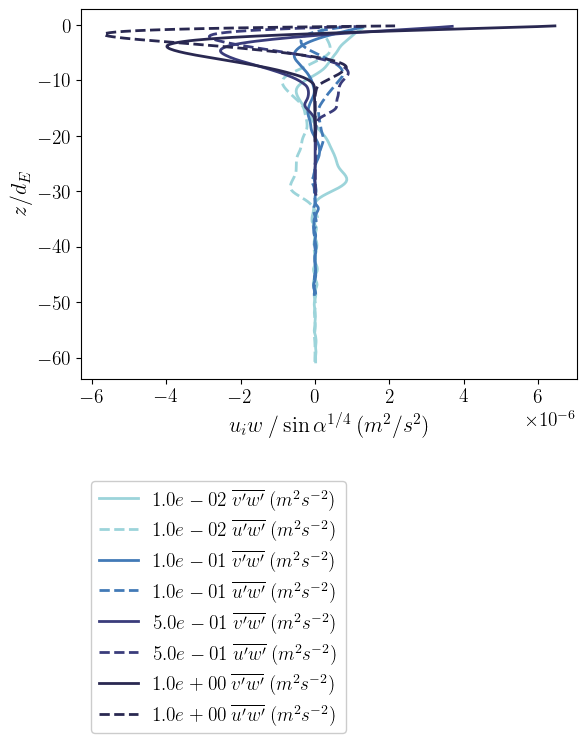
\includegraphics[trim={0 7.5cm 0 0},clip,width=\textwidth]{Figures/momflux_cmp_slope_46h_tav13_slopescale_z_profile.png}
        \centering 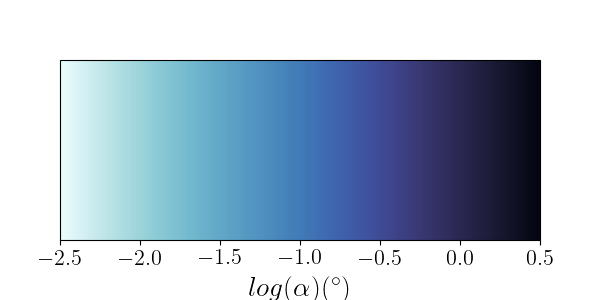
\includegraphics[width=0.7\textwidth,trim={1cm 0cm 1cm 5cm}, clip]{Figures/colorbar_slope.png}
    \end{minipage}
    \caption{Scaled vertical profile of (a,b) heat flux and (c,d) momentum flux averaged over the last inertial period for (a,c) temperature cases and (b,d) slope cases. Momentum flux is expressed in two components:  $\overline{u'w'}$ (dashed) and $\overline{v'w'}$ (solid).} 
    %Change vertical axis limits
    %Change all to centered on 43h and averaged 13h
    \label{fig:Scaled_flux_profiles}
\end{figure}

\begin{figure}[H]
    \centering
    \begin{minipage}{0.5\textwidth}
        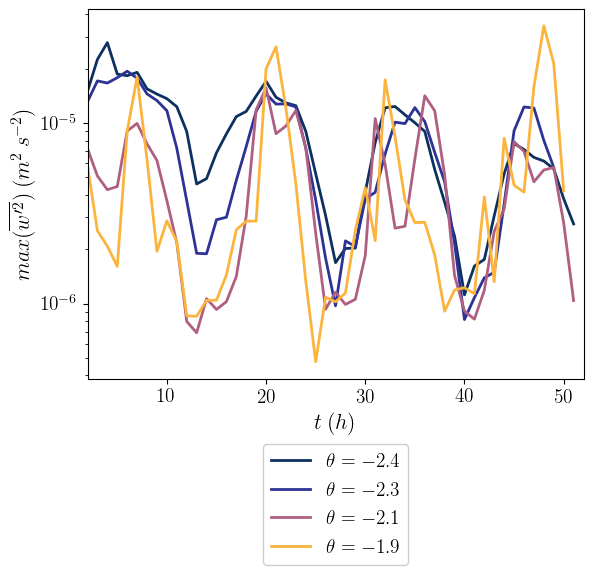
\includegraphics[width=\textwidth]{Figures/w2_max_cmp_dT_t.png}
    \end{minipage}%
    \begin{minipage}{0.5\textwidth}
        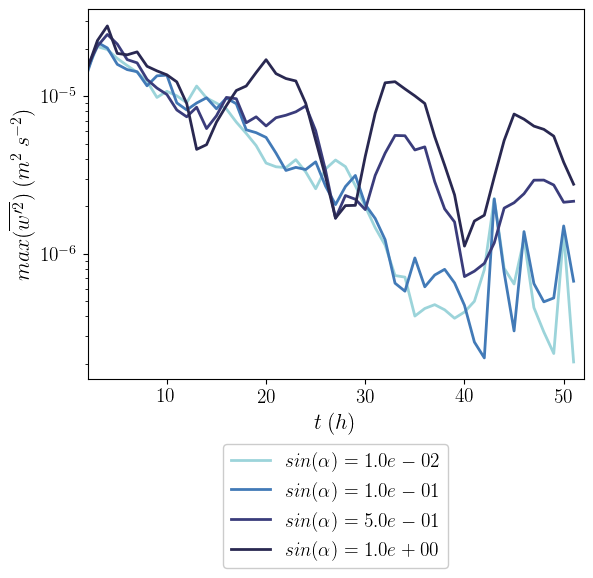
\includegraphics[width=\textwidth]{Figures/w2_max_cmp_dalpha_t.png}
    \end{minipage}
    \caption{Timeseries of maximum vertical velocity fluctuation per hour for (a) thermal driving cases and (b) slope cases.}
    \label{fig:max_w2_timeseries}
\end{figure}

\begin{figure}[H]
    \centering
    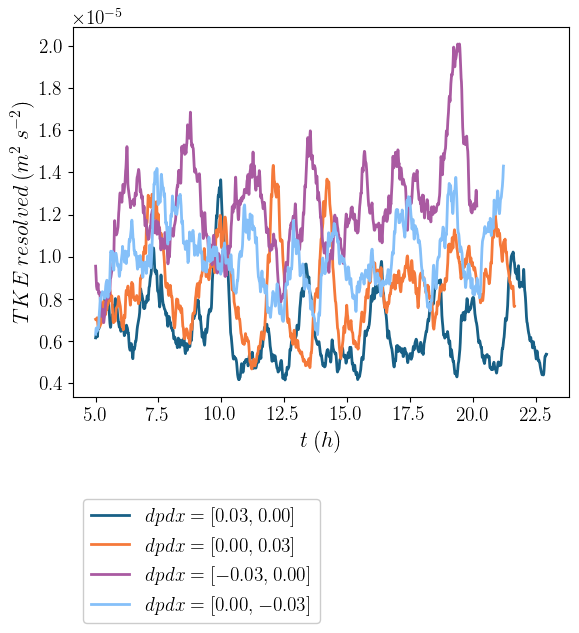
\includegraphics[width=0.5\textwidth]{Figures/e_res_cmp_dpdy_dpdx_t.png}
    \caption{Resolved turbulent kinetic energy as a function of pressure gradient orientation under 0.1$^{\circ}$ slope.}
    \label{fig:e_orientation}
\end{figure}

\begin{figure}[H]
    \centering
    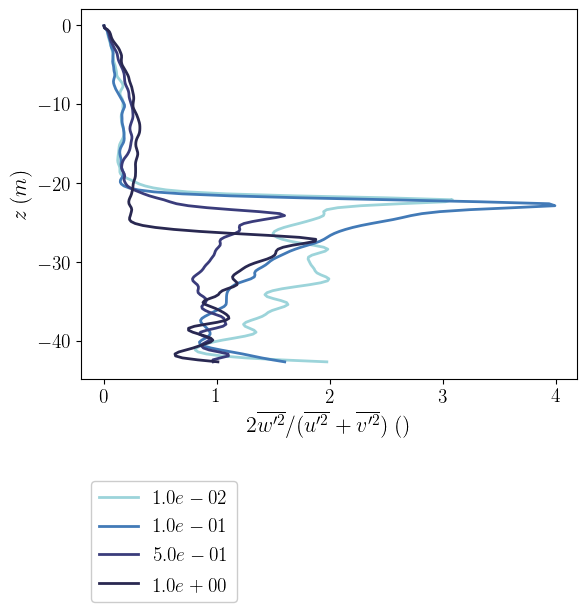
\includegraphics[width=0.5\textwidth]{Figures/vel_var_ratio_cmp_dslope_40hr_tav1_z_profile.png}
    \caption{Ratio of vertical to horizontal velocity variance for slope-varying simulations.}
    \label{fig:vel_var_ratio}
\end{figure}

\begin{figure}[H]
    \centering
    \begin{minipage}{0.5\textwidth}
        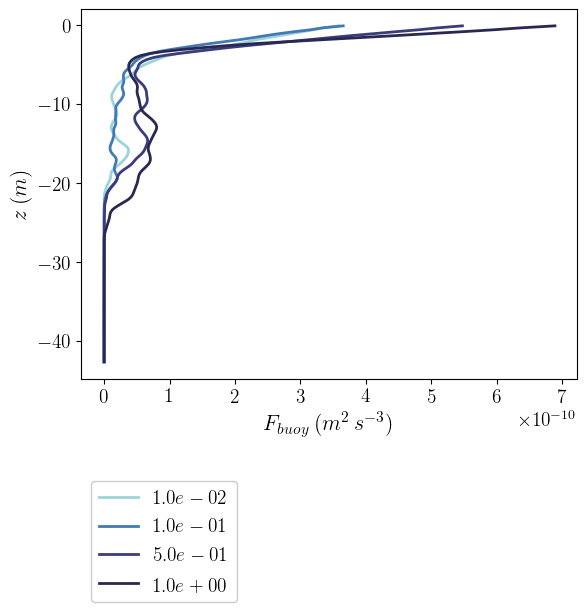
\includegraphics[trim={0 4.5cm 0 0},clip, width=\textwidth]{Figures/Fbuoy_cmp_dslope_40hr_tav1_z_profile.png}
    \end{minipage}%
    \begin{minipage}{0.5\textwidth}
        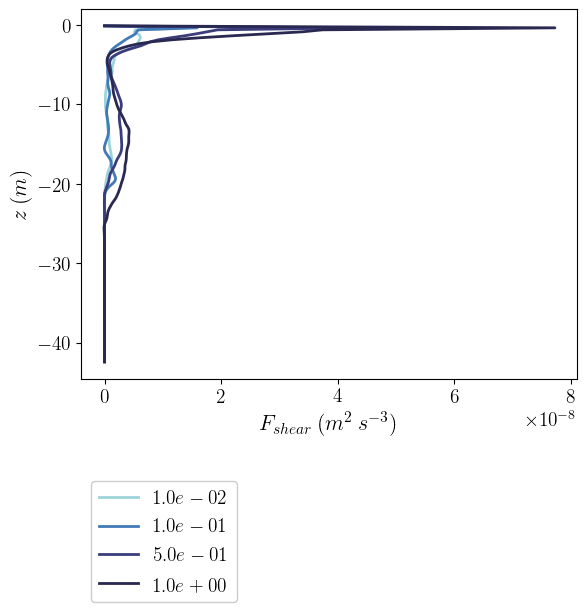
\includegraphics[trim={0 4.5cm 0 0},clip, width=\textwidth]{Figures/Fshear_cmp_dslope_40hr_tav1_z_profile.png}
    \end{minipage}
    \caption{TKE production by (a) buoyancy and (b) shear for slope-varying simulations.}
    \label{fig:tke}
\end{figure}

\begin{figure}[H]
    \centering
    \begin{minipage}{0.5\textwidth}
        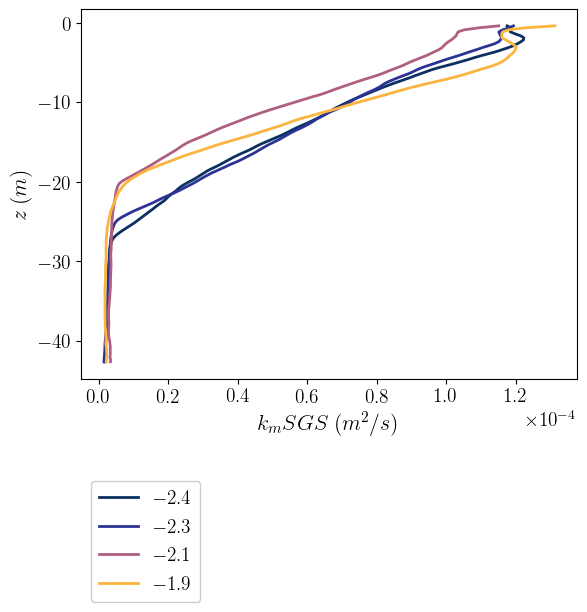
\includegraphics[trim={0 4.5cm 0 0},clip, width=\textwidth]{Figures/km_cmp_dT_44h_tav12_z_profile.png}
    \end{minipage}%
    \begin{minipage}{0.5\textwidth}
        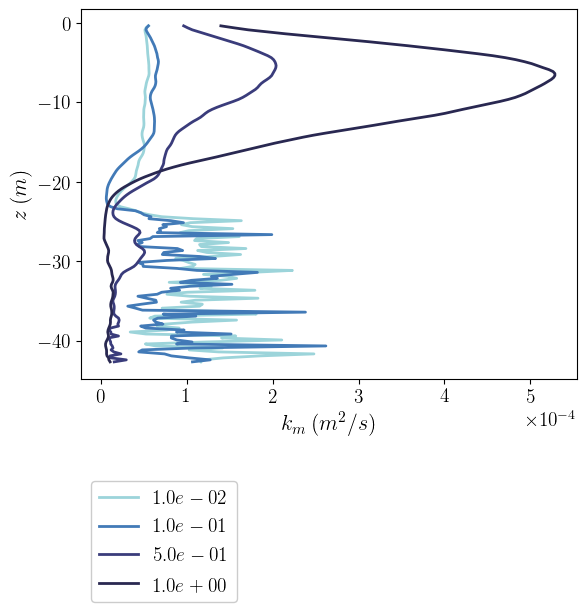
\includegraphics[trim={0 4.5cm 0 0},clip, width=\textwidth]{Figures/km_cmp_slope_46h_tav12_z_profile.png}
    \end{minipage}
    \caption{Effective vertical diffusivity for momentum flux from (a) thermal driving simulations and (b) slope-varying simulations.}
    \label{fig:km}
\end{figure}